\documentclass[12pt, a4paper]{article}
\usepackage{graphicx}
\graphicspath{ {./imgs/} }
\usepackage{float}
\usepackage{listings}
\usepackage{color}

\definecolor{codegreen}{rgb}{0,0.6,0}
\definecolor{codegray}{rgb}{0.5,0.5,0.5}
\definecolor{codeorange}{rgb}{1,0.49,0}
\definecolor{backcolour}{rgb}{0.95,0.95,0.96}

\lstset{
  backgroundcolor=\color{backcolour},   
  commentstyle=\color{codegray},
  keywordstyle=\color{codeorange},
  numberstyle=\tiny\color{codegray},
  stringstyle=\color{codegreen},
  basicstyle=\ttfamily\footnotesize,
  breakatwhitespace=false,         
  breaklines=true,                 
  captionpos=b,                    
  keepspaces=true,                 
  numbers=left,                    
  numbersep=5pt,                  
  showspaces=false,                
  showstringspaces=false,
  showtabs=false,                  
  tabsize=2,
  xleftmargin=10pt,
}
\renewcommand{\lstlistingname}{Code}

\counterwithin{figure}{section}

%to write code:
%\begin{lstlisting}[language=java, caption={my caption}]
%    
%\end{lstlisting}

%to insert an image
%\begin{figure}[H]
%  \centering
%  \includegraphics[width=\columnwidth]{img.png}
%  \caption{description of the image}
%\end{figure}

\setcounter{section}{-1}

\title{Web Architectures - Delivery 4 v2}
\author{Marrocco Simone}

\begin{document}
  \maketitle
  \begin{figure}[H]
    \centering
    
\includegraphics[scale=0.35]{unitn.png}
  \end{figure}
  \tableofcontents
  %\pagebreak

  \section{Differences to the previous version}
  In the previous version it was not clear the role of the Business Delegate, which led to confusing parts mix between backend and frontend, like html being served from the server or html generating functions in the business delegate class (which was wrongly named Facade, leading to more confusion). After discussing with the professor, the code is now much more understandable and the various roles better divided. It was removed from the backend the HTML parts, and in the frontend it was correctly added a Business Delegate which just exposes the backend methods. 

  For this document, the difference is in the Front End chapter, which substitutes the previous chapters "Html Presentation" and "Client Tomcat" and where the new Front End part is explained. The architecture image was also updated. We hope the new version is clearer. 

  \pagebreak
  \section{The assignment}

  The scope of this assignment is creating a web application backed by Enterprise Java Beans (EJBs) that interacts with a database via Java Entities to show a web page shown by a separeted server (in a distributed fashion).

  \section{Database}

  The database has three entities (Students, Courses and Teachers) and two relationships (Student-Courses is N:M and Courses-Teachers is 1:1). Here is how the schema was created.

  \begin{figure}[H]
    \centering
    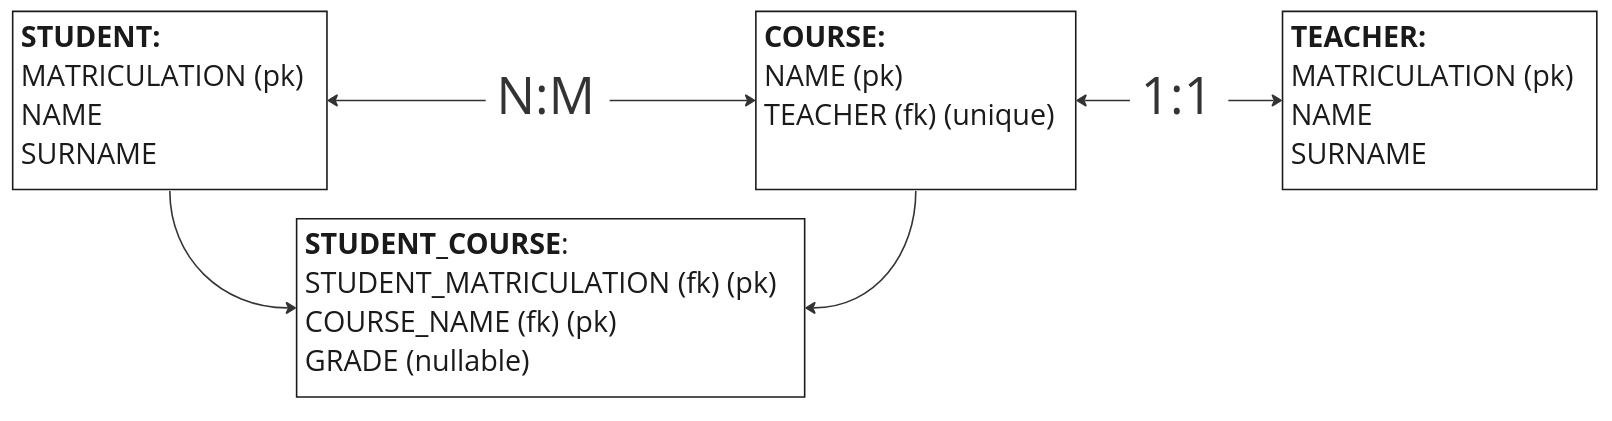
\includegraphics[width=\columnwidth]{db_schema.png}
    \caption{The database schema}
  \end{figure}

  While Teachers and Courses have a 1:1 relationship and so could be represented in a single table, it was decided to divide them for better mantenability in case in the future it is wanted to update this relationship to a 1:N one. The uniqueness of the relationship is saved in the foreign key of Course.

  It was also created a join table between Students and Courses in order to save their relationship and its Grade column.

  In particular, the choice of using Course.Name as primary key will help us later in the queries we need to execute, even if may not be the optimal choice in case we have multiple courses with the same name (we will suppose we won't, for now).

  At the end of this document, the queries used to initialize the database will be provided.

  \section{Architecture}

  Our architecture will try to be as modular as possible, so to be better scalable and mantainable. We will have three main servers: the one that serves the client; the one that handles the business logic; and the H2 database server. The database was linked to the Wildfly server via modifications in the standalone.xml file. The Clients connects to the Server using JNDI.

  \begin{figure}[H]
    \centering
    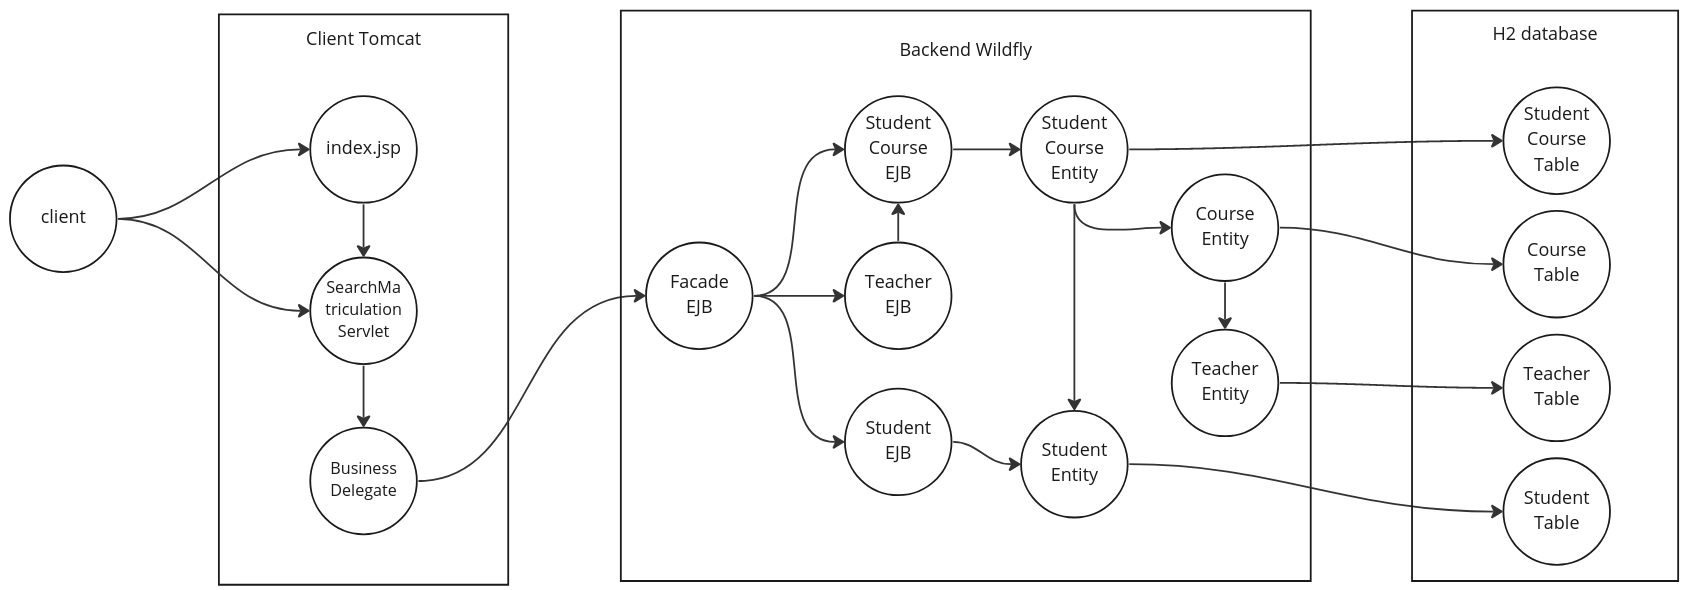
\includegraphics[width=\columnwidth]{architecture.png}
    \caption{The distributed architecture}
  \end{figure}

  In the image, we can see how every bean and entity interacts with each other. We will explain later how each one does.

  \pagebreak
  \section{Entities}

  Entities are our link between the business logic and the database. They allow us to write much simpler queries and get data in a Java-like fashion. We will now look how they are interconnected.

  For each entity, here we will omit the standard constructors, the getters/setters and the equals/hashCode, but they are present in the full code inside the project. These functions are auto generated from our IDE IntelliJ.

  \subsection{The Student Entity}
  \begin{lstlisting}[language=java, caption={The Student Entity}]
    @Entity
    @Table(name = "STUDENT")
    public class StudentEntity implements Serializable {
      @Id
      @Column(name = "MATRICULATION", nullable = false)
      @GeneratedValue(strategy = GenerationType.IDENTITY)
      private Integer matriculation;
      @Column(name = "NAME", nullable = false)
      private String name;
      @Column(name = "SURNAME", nullable = false)
      private String surname;
    }
  \end{lstlisting}

  This entity (and the next one) are very basics, since they are just a translation of their schema into Java code. We can see how we are telling the Dependecy Injector that all the fields are not nullable (like we did in the database schema).

  \pagebreak
  \subsection{The Teacher Entity}
  \begin{lstlisting}[language=java, caption={The Teacher Entity}]
    @Entity
    @Table(name = "TEACHER")
    public class TeacherEntity implements Serializable {
      @Id
      @Column(name = "MATRICULATION", nullable = false)
      @GeneratedValue(strategy = GenerationType.IDENTITY)
      private Integer matriculation;
      @Column(name = "NAME", nullable = false)
      private String name;
      @Column(name = "SURNAME", nullable = false)
      private String surname;
    }
  \end{lstlisting}

  \subsection{The Course Entity}
  \begin{lstlisting}[language=java, caption={The Course Entity}]
    @Entity
    @Table(name = "COURSE")
    public class CourseEntity implements Serializable {
      @Id
      @Column(name = "NAME", nullable = false)
      private String name;

      @JoinColumn(name = "TEACHER", nullable = false)
      @OneToOne(cascade = {CascadeType.REMOVE})
      private TeacherEntity teacher;
    }
  \end{lstlisting}

  Here we can see how we wrote the foreign key column Teacher as a JoinColumn: what this does is allowing the code to automatically join the tables and give us the already complete object it references (in this case the TeacherEntity and not a simple Integer) instead of having us manually search for it (similar to Mongoose.populate for MongoDb in Javascript). This will be really useful for later, since we won't need many WHERE clauses in the queries. We also add the Cascade property to eliminate the Course record if the corresponding Teacher is eliminated (although we won't operate such functions).

  \pagebreak
  \subsection{The StudentCourse Entity}
  \begin{lstlisting}[language=java, caption={The StudentCourse Entity}]
    @Entity
    @Table(name = "STUDENT_COURSE")
    public class StudentCourseEntity implements Serializable {
      @Id
      @JoinColumn(name = "STUDENT_MATRICULATION", nullable = false)
      @ManyToOne
      private StudentEntity student;
      @Id
      @JoinColumn(name = "COURSE_NAME", nullable = false)
      @ManyToOne
      private CourseEntity course;
      @Column(name = "GRADE", nullable = true)
      private Integer grade;
    }
  \end{lstlisting}

  Here we do the same thing with the columns StudentMatriculation and CourseName, only this time with a ManyToOne relationship instead of a OneToOne one. This is because we could have many time the same student and/or the same course. We can also see how the Grade column is nullable.

  \pagebreak
  \section{EJBs}

  For our EJBs, we need first to think about our logic: what we want to achieve and which queries we need. We need to create two pages: each one asks us the anagraphical data of a student, given its matriculation number, and then either the list of its courses and their grades or the list of its professors. We can see how to general request is simply a search on the Student table based on the matriculation number, while the specific ones need their specific queries.

  On the naming convention: we call the interface by a simple name (like Students) and their bean implementation as the same name plus "EJB" (like StudentsEJB). In the code below we won't show the interface, since it is easily guessable (they are made of the public EJB methods).

  \subsection{StudentEJB}
  For the general one, we can create a Student EJB that does exactly that: a simple query that returns our searched Student. If we receive the error NoResultException, it means the query was unsuccessful: we return null and make the caller deal with that.
  
  \begin{lstlisting}[language=java, caption={StudentsEJB}]
    @Stateless
    @Local(Students.class)
    public class StudentsEJB implements Students{
      @PersistenceContext(unitName="default")
      private EntityManager entityManager;

      @Override
      public StudentEntity getSingleStudent(int matriculation){
        try {
          Query q = entityManager.createQuery("From StudentEntity where matriculation = " + matriculation);
          StudentEntity s = (StudentEntity) (q.getSingleResult());
          return s;
        } catch (NoResultException e) {
          System.out.println("Student was not found");
          return null;
        }
      }
    }
  \end{lstlisting}

  \subsection{StudentCourseEJB}
  For the search of a student's courses, normally we would need to join the three tables Student, Course and StudentCourse. However, we can do something better: the student matriculation number and the name of the course are both fields already present in our StudentCourse table. So the query is as easy as the one before.

  \begin{lstlisting}[language=java, caption={StudentCourseEJB}]
    @Stateless
    @Local(StudentCourse.class)
    public class StudentCourseEJB implements StudentCourse {
      @PersistenceContext(unitName="default")
      private EntityManager entityManager;

      @Override
      public List<StudentCourseEntity> getStudentCourses(int matriculation) {
        try {
          Query q = entityManager.createQuery(
            "From StudentCourseEntity where student.matriculation = " + matriculation
          );
          List<StudentCourseEntity> sc = q.getResultList();
          if (sc.isEmpty()) System.out.println("StudentCourse is empty");
          return sc;
        } catch (NoResultException e) {
          System.out.println("StudentCourse was not found");
          return null;
        }
      }
    }
  \end{lstlisting}

  If instead we wanted the class Course to have a numerical ID and use it as a foreign key inside StudentCourse, the query would still remain the same: as we said before, StudentCourseEntity already has as one of its fields not the simple foreign key but the entire reference object, as we will show with the next query.

  \pagebreak
  \subsection{TeachersEJB}

  \begin{lstlisting}[language=java, caption={TeachersEJB}]
    @Stateless
    @Local(Teachers.class)
    public class TeachersEJB implements Teachers {
      @PersistenceContext(unitName="default")
      private EntityManager entityManager;

      Context ctx;
      StudentCourse studentCourseEJB;
      public void ejbCreate() {
        try {
          studentCourseEJB = (StudentCourse) ServiceLocator.getService("java:module/StudentCourseEJB!it.marrocco.marroccoass4_2server.ejb.StudentCourse");
        } catch (NamingException e) {
          throw new RuntimeException(e);
        }
      }

      @Override
      public List<TeacherEntity> getStudentTeachers(int matriculation) {
        List<StudentCourseEntity> sc = studentCourseEJB.getStudentCourses(matriculation);
        if (sc == null) return null;
        List<TeacherEntity> t = new ArrayList<>();
        for (StudentCourseEntity s : sc) {
            t.add(s.getCourse().getTeacher());
        }
        return t;
      }
    }
  \end{lstlisting}

  Since the StudentCourseEntity already has the full referenced object, we do not need a new query: we can use the same one used before and just go a little bit deeper in the resulted object. We start by creating a lookup link to our StudentCourseEJB at the creation of this bean, done in the function ejbCreate, then we call its method and extract from each StudentCourseEntity the referenced TeacherEntity (this is why in the architecture TeacherEJB did not reach out to TeacherEntity directly).

  We can see here a strange thing, and another one across all this beans: instead of doing a classic lookup we use something called ServiceLocator, and all our beans are locals! The reason is simple: we are using well established patterns.

  \pagebreak
  \section{Patterns}
  Patterns are a well known and studied way to resolve common problems. Here we show how we are using two of them. We are using two more, DTO and Business delegates, but we will talk about them later when distributing the application.
  
  \subsection{ServiceLocator}
  Context Lookup are heavy in resources to execute: most of the time it may happen that we look up multiple times the same bean. It is much more efficient to delegate all the lookups to a single class which can cache them for multiple calls without much overhead.
  \begin{lstlisting}[language=java, caption={ServiceLocator}]
    public class ServiceLocator {
    private static HashMap<String, Object> cache;

    static {
      cache = new HashMap<String, Object>();
    }

    public static Object getService(String jndiName) throws NamingException {
      Object service = cache.get(jndiName);
      if (service == null) {
        InitialContext context = new InitialContext();
        service = context.lookup(jndiName);
        cache.put(jndiName, service);
      }
      return service;
    }
}
  \end{lstlisting}
  
  \pagebreak
  \subsection{FacadeEJB}
  It is not ideal having the client interface with multiple beans: what we can do is create a single Remote EJB which proxies all the function we need to expose, so that the client only needs to connect to as few EJB as possible.
  \begin{lstlisting}[language=java, caption={FacadeEJB}]
    @Stateless
    @Remote(Facade.class)
    public class FacadeEJB implements Facade {
      StudentCourse studentCourseEJB;
      Teachers teachersEJB;
      Students studentsEJB;
      public void ejbCreate() {
        try {
          studentCourseEJB = (StudentCourse) ServiceLocator.getService("java:module/StudentCourseEJB!it.marrocco.marroccoass4_2server.ejb.StudentCourse");
          teachersEJB = (Teachers) ServiceLocator.getService("java:module/TeachersEJB!it.marrocco.marroccoass4_2server.ejb.Teachers");
          studentsEJB = (Students) ServiceLocator.getService("java:module/StudentsEJB!it.marrocco.marroccoass4_2server.ejb.Students");
        } catch (NamingException e) {
          throw new RuntimeException(e);
        }
      }
  
      @Override
      public StudentEntity getSingleStudent(int matriculation) {
        return studentsEJB.getSingleStudent(matriculation);
      }
  
      @Override
      public List<StudentCourseEntity> getStudentCourses(int matriculation) {
        return studentCourseEJB.getStudentCourses(matriculation);
      }
  
      @Override
      public List<TeacherEntity> getStudentTeachers(int matriculation) {
        return teachersEJB.getStudentTeachers(matriculation);
      }
    }\end{lstlisting}

  %\pagebreak
\section{Html Presentation}
Now we need to convert the Entities we have into html.
First we create the index.jsp file, which is a simple form that has a field for the matriculation and two checks, one for each page, to choose what to generate: in this way, we can test both pages simultaneously (the real version would have two different buttons that redirects to two different pages).

\begin{figure}[H]
  \centering
  
\includegraphics[width=\columnwidth]{index.png}
  \caption{The starting page}
\end{figure}

The form will redirect to our servlet, which will call a special bean, HtmlElementEBJ, used to create the elements we need for our page. This bean will use the FacadeEJB to call its method, parse the results and transform them into a ready-to-use html element. This is known as Business Delegate: by dealing with the business implementation in this bean, we can free the client part from knowing the backend, instead of referencing FacadeEJB all across the frontend. The shown version uses a local FacadeEJB: we will see later how to convert it to a remote call.

\begin{lstlisting}[language=java, caption={Servlet doPost}]
    public void doPost(HttpServletRequest request, HttpServletResponse response) throws IOException {
      int matriculation;
      try {
        matriculation = Integer.parseInt(request.getParameter("matriculation"));
      } catch (NumberFormatException e) {
        response.sendRedirect("");
        return;
      }
      boolean showStudentPage = request.getParameter("studentPage") != null;
      boolean showAdvisoryPage = request.getParameter("advisoryPage") != null;

      String html = "";
      String name;
      try {
        name = "java:module/HtmlElementsEJB!it.marrocco.h2ejbdemo.ejb.HtmlElements";
        HtmlElements htmlElementsEJB = (HtmlElements) ServiceLocator.getService(name);

        if (showStudentPage) html += htmlElementsEJB.getStudentPageElement(matriculation);
        if (showAdvisoryPage) html += htmlElementsEJB.getAdvisoryPageElement(matriculation);
      } catch (NamingException e) {
        html += "<h1>" + e.getMessage() + "</h1>";
      }

      response.setContentType("text/html");
      PrintWriter out = response.getWriter();
      out.println("<html><head><title>Matriculation "+matriculation+"</title></head><body>");
      out.println(html);
      out.println("<a href='index.jsp'>Go back</a>");
      out.println("</body></html>");
      out.close();
    }
  \end{lstlisting}

\begin{lstlisting}[language=java, caption={HtmlElementsEJB}]
    @Stateless
    @Local(HtmlElements.class)
    public class HtmlElementsEJB implements HtmlElements{
      Facade facadeEJB;
      public void ejbCreate() {
        try {
          facadeEJB = (Facade) ServiceLocator.getService("java:module/FacadeEJB!it.marrocco.h2ejbdemo.ejb.Facade");
        } catch (NamingException e) {
          throw new RuntimeException(e);
        }
      }
  
      @Override
      public String formatStudentEntity(StudentEntity s) {
        return "<h1>" + s.getSurname() + " " + s.getName() + " (" + s.getMatriculation() + ")</h1>";
      }
  
      @Override
      public String getStudentPageElement(int matriculation) {
        StudentEntity s = facadeEJB.getSingleStudent(matriculation);
        if (s == null) return "<h1>Student was not found</h1>";
        String html = formatStudentEntity(s);
        html += "<h2>Courses:</h2>";
        try {
          html += "<ul>";
          List<StudentCourseEntity> sc = facadeEJB.getStudentCourses(matriculation);
          if (sc == null) return "<h1>Error getting the Student Courses</h1>";
          for (StudentCourseEntity c : sc) {
            html += "<li>" + c.getCourse().getName();
            if(c.getGrade() != null)
              html +=  " (grade = " + c.getGrade() + ")";
            html += "</li>";
          }
          html += "</ul>";
        } catch (Exception e ) {
          System.out.println("error: " + e.getMessage());
          html += "<h3>error<h3>";
        }
        return html;
    }

    @Override
    public String getAdvisoryPageElement(int matriculation) {
        StudentEntity s = facadeEJB.getSingleStudent(matriculation);
        if (s == null) return "<h1>Student was not found</h1>";
        String html = formatStudentEntity(s);
        html += "<h2>Advisors:</h2>";
        try {
          html += "<ul>";
          List<TeacherEntity> sc = facadeEJB.getStudentTeachers(matriculation);
          if (sc == null) return "<h1>Error getting the Student Teachers</h1>";
          for (TeacherEntity t : sc) {
            html += "<li>" + t.getSurname() + " " + t.getName() + "</li>";
          }
          html += "</ul>";
        } catch (Exception e ) {
          System.out.println("error: " + e.getMessage());
          html += "<h3>error<h3>";
        }
        return html;
    }
    }
  \end{lstlisting}

\begin{figure}[H]
  \centering
  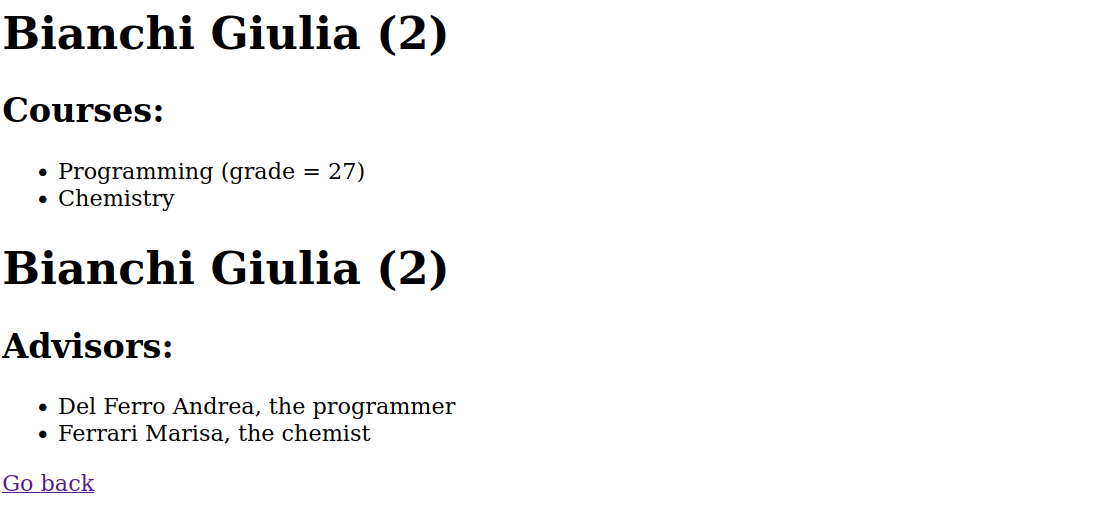
\includegraphics[width=\columnwidth]{full_page.png}
  \caption{The servlet page when both checks are set, showing both requested pages}
\end{figure}

\begin{figure}[H]
  \centering
  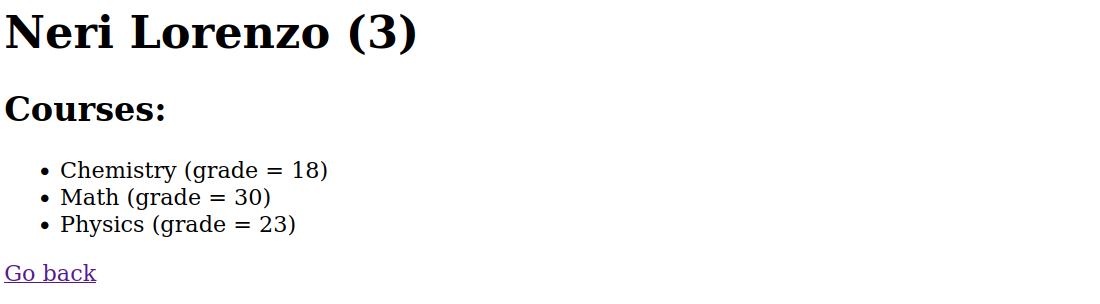
\includegraphics[width=\columnwidth]{only_one_page.png}
  \caption{The servlet page with only the courses page}
\end{figure}

\begin{figure}[H]
  \centering
  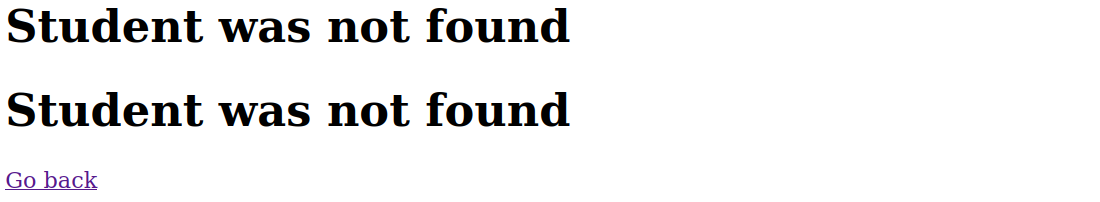
\includegraphics[width=\columnwidth]{no_student_found.png}
  \caption{The servlet page when a non existant student is searched}
\end{figure}

\pagebreak
\section{Client Tomcat}
The objective of this assignment was to separate in a distributed system the backend logic and the frontend presentation. Fortunately, this operation is not much complicated.
In the client server, what we need from the backend is:
\begin{itemize}
  \item  the entities, without the injection code;
  \item  the Facade interface, which will send us the serialized entities objects (DTO);
  \item  the HtmlElementsEJB, where we need to change the FacadeEJB lookup adress and substitute the method ebjCreate to a constructor;
  \item  the ServiceLocator, where in the context creation we need to add the Jndi properties to connect to the Wildfly server;
  \item  the index.jsp;
  \item  our servlet, where instead of using a lookup for the HtmlElementsEJB we need to instantiate the bean ourself in the code.
\end{itemize}

\begin{lstlisting}[language=java, caption={The new HtmlElementsEJB}]
    public class HtmlElementsEJB implements HtmlElements{
      Facade facadeEJB;
      public HtmlElementsEJB() {
        try {
          facadeEJB = (Facade) ServiceLocator.getService("ejb:/H2EJBDemo-1.0-SNAPSHOT/FacadeEJB!it.marrocco.h2ejbdemo.ejb.Facade");
        } catch (NamingException e) {
          System.out.println("Naming exception: " + e.getMessage());
          e.printStackTrace();
          throw new RuntimeException(e);
        }
      }
      // same methods as before
    }
  \end{lstlisting}

\begin{lstlisting}[language=java, caption={The new ServiceLocator}]
    public class ServiceLocator {
      private static HashMap<String, Object> cache;

      static {
        cache = new HashMap<String, Object>();
      }

      private static Properties getJndiProperties() {
        Properties jndiProperties=new Properties();
        jndiProperties.put(Context.INITIAL_CONTEXT_FACTORY, "org.wildfly.naming.client.WildFlyInitialContextFactory");
        jndiProperties.put(Context.PROVIDER_URL,"http-remoting://localhost:8080");
        return jndiProperties;
      }

      public static Object getService(String jndiName) throws NamingException {
        Object service = cache.get(jndiName);
        if (service == null) {
          InitialContext context = new InitialContext(getJndiProperties());
          service = context.lookup(jndiName);
          cache.put(jndiName, service);
        }
        return service;
      }
    }
  \end{lstlisting}

\begin{lstlisting}[language=java, caption={The new Servlet doPost}]
    public void doPost(HttpServletRequest request, HttpServletResponse response) throws IOException {
      // same parameters controlls as before
      String html = "";
      try {
        HtmlElements htmlElementsEJB = new HtmlElementsEJB();

        if (showStudentPage) html += htmlElementsEJB.getStudentPageElement(matriculation);
        if (showAdvisoryPage) html += htmlElementsEJB.getAdvisoryPageElement(matriculation);
      } catch (Exception e) {
        System.out.println("Error in fetching data");
        html += "<h1>Error in fetching data</h1>";
      }
      // same html creation as before
    }
  \end{lstlisting}

  \pagebreak
\section{Front End}
\subsection{Business Delegate}

The team working on the frontend needs to have ready to use functions, without having to know how the backend works or how to connect to it. This is why we create a Business Delegate, a class made by the backend team which gives the functions useful for the frontend application.

In our case, the backend team need to give two things. The first is a subset of the package used in the server containing the Facade interface and the Entities classes. This is needed because the backend methods will return these classes, which are just objects with some fields, getters/setters and equals/hashCode functions (cleaned of the extra injections used in the backend). They are implementing Serializable, which makes easy for them to be shared remotely (DTO). To make JNDI work, we need to put these files, which are in common with the server, in the same package structure as the server itself, otherwise the connection will return the ClassNotFoundException. 
\footnote{https://stackoverflow.com/questions/13701041/remote-ejb-call-class-not-found-\\exception/13703265}

The second thing the backend team will give to the frontend one is a folder containing the business delegate class and a service locator. The frontend team will need only to interface with the business delegate class to do their job. The service locator for the client is not used to find the different EJBs inside the project, but to interface with the server: in this case, we need the \textit{InitialContext} to have some properties to tell him where to connect (properties given by the function \textit{getJndiProperties()}). We can see how also here the Service Locator is a Singleton.

\begin{figure}[H]
  \centering
  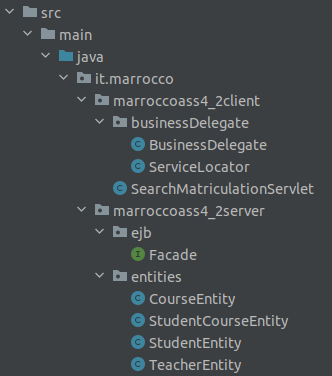
\includegraphics[width=0.3\columnwidth]{client_folder_structure.png}
  \caption{The structure of the Client project}
\end{figure}

\pagebreak
\begin{lstlisting}[language=java, caption={BusinessDelegate}]
  public class BusinessDelegate {
      Facade facadeEJB;
      public BusinessDelegate() {
          try {
              String jndiName = "ejb:/MarroccoAss4_2-Server-1.0-SNAPSHOT/FacadeEJB!it.marrocco.marroccoass4_2server.ejb.Facade";
              facadeEJB = (Facade) ServiceLocator.getService(jndiName);
          } catch (NamingException e) {
              System.out.println("Naming exception: " + e.getMessage());
              e.printStackTrace();
              throw new RuntimeException(e);
          }
      }

      public StudentEntity getSingleStudent(int matriculation) {
          return facadeEJB.getSingleStudent(matriculation);
      }

      public List<StudentCourseEntity> getStudentCourses(int matriculation) {
          return facadeEJB.getStudentCourses(matriculation);
      }

      public List<TeacherEntity> getStudentTeachers(int matriculation) {
          return facadeEJB.getStudentTeachers(matriculation);
      }
  }
\end{lstlisting}

\pagebreak
\begin{lstlisting}[language=java, caption={Client ServiceLocator}]
  public class ServiceLocator {
      private static HashMap<String, Object> cache;

      static {
          cache = new HashMap<String, Object>();
      }

      private static Properties getJndiProperties() {
          Properties jndiProperties=new Properties();
          jndiProperties.put(Context.INITIAL_CONTEXT_FACTORY, "org.wildfly.naming.client.WildFlyInitialContextFactory");
          jndiProperties.put(Context.PROVIDER_URL,"http-remoting://localhost:8080");
          jndiProperties.put(Context.URL_PKG_PREFIXES, "org.jboss.ejb.client.naming");
          jndiProperties.put("jboss.naming.client.ejb.context", true);

          return jndiProperties;
      }

      public static Object getService(String jndiName) throws NamingException {
          Object service = cache.get(jndiName);
          if (service == null) {
              InitialContext context = new InitialContext(getJndiProperties());
              service = context.lookup(jndiName);
              cache.put(jndiName, service);
          }
          return service;
      }
  }
\end{lstlisting}

\pagebreak
\subsection{Html Pages}
First we create the index.jsp file, which is a simple form that has a field for the matriculation number and two checks, one for each page, to choose what to get from the server.

The form will redirect to our servlet, which will take the matriculation number from the request body. It will then instantiate the class BusinessDelegate made by the backend team in the \textit{init()} method, call its functions to get the data necessary from the server and use it to create HTML parts.

\begin{lstlisting}[language=java, caption={SearchMatriculationServlet}]
  @WebServlet(name = "searchMatriculation", value = "/searchMatriculation")
  public class SearchMatriculationServlet extends HttpServlet {
      BusinessDelegate bd;
  
      @Override
      public void init() {
          try {
              bd = new BusinessDelegate();
              System.out.println("Connection working");
          } catch(RuntimeException e) {
              System.out.println("Cannot get connection to server");
          }
      }
  
      public String formatStudentEntity(StudentEntity s) {
          return "<h1>" + s.getSurname() + " " + s.getName() + " (" + s.getMatriculation() + ")</h1>";
      }
  
      public String getStudentPageElement(int matriculation) {
          StudentEntity s = bd.getSingleStudent(matriculation);
          if (s == null) return "<h1>Student was not found</h1>";
          String html = formatStudentEntity(s);
          html += "<h2>Courses:</h2>";
          try {
              html += "<ul>";
              List<StudentCourseEntity> sc = bd.getStudentCourses(matriculation);
              if (sc == null) return "<h1>Error getting the Student Courses</h1>";
              for (StudentCourseEntity c : sc) {
                  html += "<li>" + c.getCourse().getName();
                  if(c.getGrade() != null)
                      html +=  " (grade = " + c.getGrade() + ")";
                  html += "</li>";
              }
              html += "</ul>";
          } catch (Exception e ) {
              System.out.println("error: " + e.getMessage());
              html += "<h3>error<h3>";
          }
          return html;
      }
  
      public String getAdvisoryPageElement(int matriculation) {
          StudentEntity s = bd.getSingleStudent(matriculation);
          if (s == null) return "<h1>Student was not found</h1>";
          String html = formatStudentEntity(s);
          html += "<h2>Advisors:</h2>";
          try {
              html += "<ul>";
              List<TeacherEntity> sc = bd.getStudentTeachers(matriculation);
              if (sc == null) return "<h1>Error getting the Student Teachers</h1>";
              for (TeacherEntity t : sc) {
                  html += "<li>" + t.getSurname() + " " + t.getName() + "</li>";
              }
              html += "</ul>";
          } catch (Exception e ) {
              System.out.println("error: " + e.getMessage());
              html += "<h3>error<h3>";
          }
          return html;
      }
  
      public void doPost(HttpServletRequest request, HttpServletResponse response) throws IOException {
          int matriculation;
          try {
              matriculation = Integer.parseInt(request.getParameter("matriculation"));
          } catch (NumberFormatException e) {
              response.sendRedirect("");
              return;
          }
          boolean showStudentPage = request.getParameter("studentPage") != null;
          boolean showAdvisoryPage = request.getParameter("advisoryPage") != null;
  
          String html = "";
          try {
              if (showStudentPage) html += getStudentPageElement(matriculation);
              if (showAdvisoryPage) html += getAdvisoryPageElement(matriculation);
          } catch (Exception e) {
              System.out.println("Error in fetching data");
              html += "<h1>Error in fetching data</h1>";
              html += "<p>"+e.getMessage()+"</p>";
          }
  
          response.setContentType("text/html");
          PrintWriter out = response.getWriter();
          out.println("<html><head><title>Matriculation "+matriculation+"</title></head><body>");
          out.println(html);
          out.println("<a href='index.jsp'>Go back</a>");
          out.println("</body></html>");
          out.close();
      }
  }
\end{lstlisting}

\pagebreak
\subsection{Pages Images}

\begin{figure}[H]
  \centering
  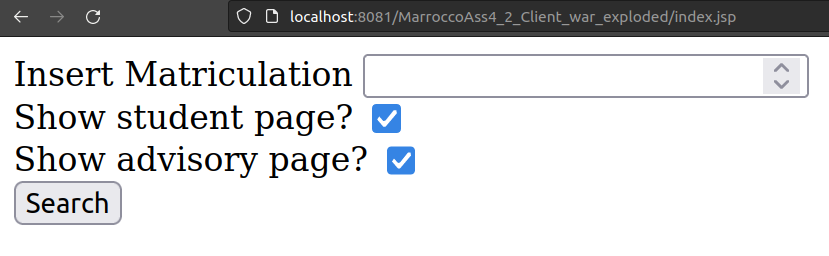
\includegraphics[width=0.7\columnwidth]{index2.png}
  \caption{The starting page}
\end{figure}

\begin{figure}[H]
  \centering
  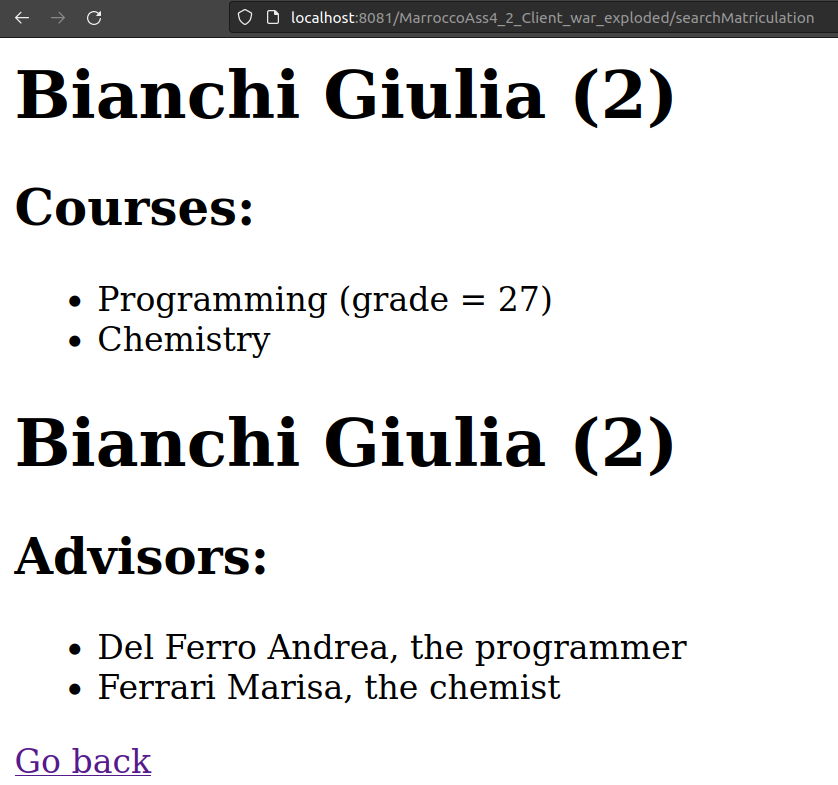
\includegraphics[width=0.7\columnwidth]{full_page2.png}
  \caption{The servlet page when both checks are set, showing both requested pages}
\end{figure}

\begin{figure}[H]
  \centering
  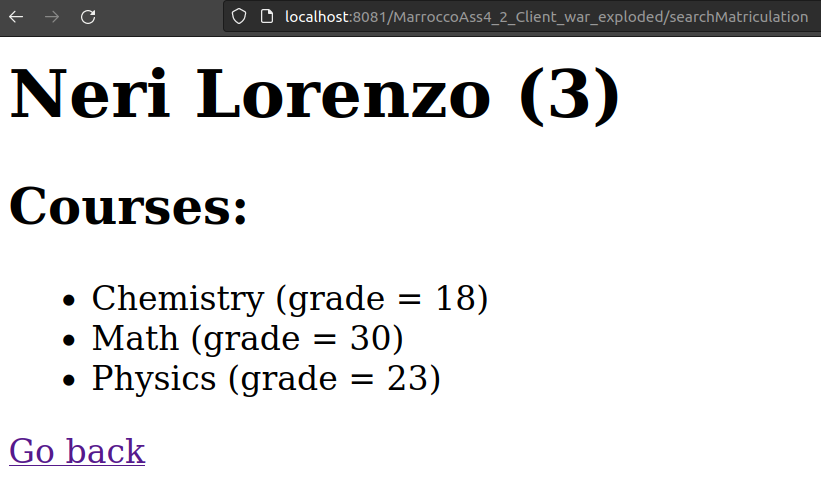
\includegraphics[width=0.7\columnwidth]{only_one_page2.png}
  \caption{The servlet page with only the courses page}
\end{figure}

\begin{figure}[H]
  \centering
  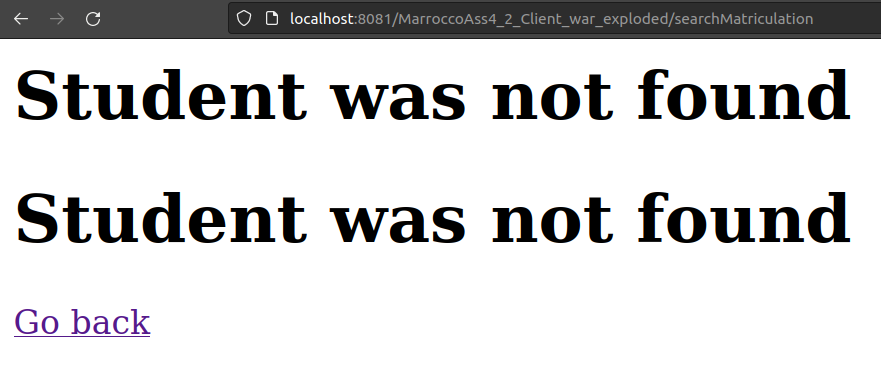
\includegraphics[width=0.7\columnwidth]{no_student_found2.png}
  \caption{The servlet page when a non existant student is searched}
\end{figure}

  \pagebreak
  \section{Appendix A: Database Initialization}
  For better debugging, in the Teachers names strings it was added a short text describing their role. Of course, it is not something that would be added in a real case scenario.

  \begin{lstlisting}[language=sql, caption={Queries to initialize the DB}]
    drop table if exists STUDENT_COURSE;
    drop table if exists COURSE;
    drop table if exists STUDENT;
    drop table if exists TEACHER;
  
    create table STUDENT (
      MATRICULATION int NOT NULL AUTO_INCREMENT, 
      NAME varchar(255) NOT NULL, 
      SURNAME varchar(255) NOT NULL,
  
      primary key (MATRICULATION)
    );
    create table TEACHER (
      MATRICULATION int NOT NULL AUTO_INCREMENT, 
      NAME varchar(255) NOT NULL, 
      SURNAME varchar(255) NOT NULL,
  
      primary key (MATRICULATION)
    );
    create table COURSE (
      NAME varchar(255) NOT NULL, 
      TEACHER varchar(255) NOT NULL UNIQUE,
  
      primary key (NAME),
      foreign key (TEACHER) references TEACHER(MATRICULATION)
    );
    create table STUDENT_COURSE (
      STUDENT_MATRICULATION int NOT NULL, 
      COURSE_NAME varchar(255) NOT NULL,
      GRADE int,
  
      primary key (STUDENT_MATRICULATION, COURSE_NAME),
      foreign key (STUDENT_MATRICULATION) references STUDENT(MATRICULATION),
      foreign key (COURSE_NAME) references COURSE(NAME)
    );
  
    insert into STUDENT values (1, 'Mario', 'Rossi');
    insert into STUDENT values (2, 'Giulia', 'Bianchi');
    insert into STUDENT values (3, 'Lorenzo', 'Neri');
    insert into STUDENT values (4, 'Rita', 'Verdi');
  
    insert into TEACHER values (1, 'Andrea, the programmer', 'Del Ferro');
    insert into TEACHER values (2, 'Giuseppe, the mathematician', 'Benedetti');
    insert into TEACHER values (3, 'Marisa, the chemist', 'Ferrari');
    insert into TEACHER values (4, 'Lucrezia, the physicist', 'Bruno');
  
    insert into COURSE values ('Programming', 1);
    insert into COURSE values ('Math', 2);
    insert into COURSE values ('Chemistry', 3);
    insert into COURSE values ('Physics', 4);
  
    insert into STUDENT_COURSE values (1, 'Programming', null);
    insert into STUDENT_COURSE values (1, 'Math', 25);
    insert into STUDENT_COURSE values (2, 'Programming', 27);
    insert into STUDENT_COURSE values (2, 'Chemistry', null);
    insert into STUDENT_COURSE values (3, 'Chemistry', 18);
    insert into STUDENT_COURSE values (3, 'Math', 30);
    insert into STUDENT_COURSE values (3, 'Physics', 23);
    insert into STUDENT_COURSE values (4, 'Physics', 30);
  
    select * from STUDENT;
    select * from TEACHER;
    select * from COURSE;
    select * from STUDENT_COURSE;
  
    select * from STUDENT, TEACHER, COURSE, STUDENT_COURSE
      where STUDENT.MATRICULATION = STUDENT_COURSE.STUDENT_MATRICULATION
      and COURSE.NAME = STUDENT_COURSE.COURSE_NAME
      and COURSE.TEACHER = TEACHER.MATRICULATION;
  \end{lstlisting}
\end{document}
